\documentclass[a4paper]{amsart}
% basics
\usepackage{a4wide} %A4 paper border
\usepackage[utf8]{inputenc}

% hyperref
\usepackage[colorlinks=true,
            raiselinks=true,
            linkcolor=MidnightBlue,
            citecolor=ForestGreen,
            urlcolor=RoyalPurple,
            plainpages=false]{hyperref}
            
% bib 
\usepackage[
bibencoding=utf8,
sorting=none,
style=numeric-comp,
backend=biber]{biblatex}
\addbibresource{refs.bib}

% graphics/color
\usepackage{graphicx}
\usepackage[usenames, dvipsnames, pdftex]{xcolor}
\usepackage{tikz}
\usetikzlibrary{arrows}

% math things
\usepackage{IEEEtrantools}
\usepackage[charter]{mathdesign}
\usepackage{amsmath} 
\usepackage{amsfonts}
\usepackage{amsthm}

\newtheorem{theorem}{Theorem}
\newtheorem{lemma}{Lemma}
\newtheorem{corollary}{Corollary}
\newtheorem{definition}{Definition}
\newtheorem{example}{Example}
\newtheorem{remark}{Remark}
\newtheorem{fact}{Fact}
\newtheorem{proposition}{Proposition}

% custom commands 
%C plus plus
\newcommand\Cpp{C\texttt{++} }

\usepackage{stmaryrd}  % because of llbracket/rrbracket
\newcommand{\segcc}[1]{\ensuremath{{\left\llbracket#1\right\rrbracket}}}

%% begin: some math stuff
\newcommand{\intcc}[1]{\ensuremath{{\left[#1\right]}}}
\newcommand{\intoc}[1]{\ensuremath{{\left]#1\right]}}}
\newcommand{\intco}[1]{\ensuremath{{\left[#1\right[}}}
\newcommand{\intoo}[1]{\ensuremath{{\left]#1\right[}}}


\newcommand{\B}{\mathbb{B}}
\newcommand{\R}{\mathbb{R}}
\newcommand{\N}{\mathbb{N}}
\newcommand{\Z}{\mathbb{Z}}

\newcommand{\pre}{{\mathrm{pre}}}
\renewcommand{\emptyset}{{\varnothing}}

% algorithm stuff
\usepackage{algorithm}
\usepackage[noend]{algpseudocode}
\algnewcommand\algorithmicinput{\textbf{Input:}}
\algnewcommand\Input{\item[\algorithmicinput]}
\algnewcommand\algorithmicoutput{\textbf{Output:}}
\algnewcommand\Output{\item[\algorithmicoutput]}
% code snippets
\usepackage{listings}
\definecolor{classes}{named}{MidnightBlue}
\definecolor{types}{named}{MidnightBlue}
\definecolor{keywords}{named}{ForestGreen}
\definecolor{strings}{named}{RoyalPurple}
%
\lstset{emph=[1]{uint32_t,abs_type,input_type,state_type},%
        emphstyle=[1]{\color{types}}%
}%
\lstset{emph=[2]{UniformGrid, 
                 Abstraction, 
                 SymbolicSet, 
                 SymbolicModel, 
                 WinningDomain, 
                 TransitionFunction, 
                 StaticController},
        emphstyle=[2]{\color{classes}}%
}%
\lstset{literate={scots::}{{{\color{classes}scots::}}}7}
% set the default code style
\lstset{
    columns=fullflexible,
    basicstyle=\ttfamily,
    frame=tb, % draw a frame at the top and bottom of the code block
    tabsize=2, % tab space width
    showstringspaces=false, % don't mark spaces in strings
    numbers=none, % display line numbers on the left
    commentstyle=\color{Gray}, % comment color
    keywordstyle=\color{keywords}, % keyword color
    stringstyle=\color{strings}, % string color
    language=C++,
}

% tabular column width
\usepackage{array}
\newcolumntype{C}{>{\centering\arraybackslash}p{2cm}}
\newcolumntype{N}{>{\centering\arraybackslash}p{1cm}}

\title{SCOTS (0.2) -- User Manual}

\author{Matthias Rungger}

\begin{document}
  \maketitle

  \addtocontents{toc}{\setcounter{tocdepth}{1}}
	\tableofcontents
	\newpage
	

\section{ToDo}

\begin{enumerate}
  \item Explain usage of the implementation using binary decision diagrams
  (BDDs) as basic data structure
  \item Provide performance tables comparing sparse matrix data structure vs BDD
  \item Support for periodic dynamics
\end{enumerate}





%\subsection{Performance Comparison}
%
% {\color{red} some initial numbers}
%
%
%Performance values for the construction of symbolic models.
%
%For the BDD performance values we distinguish with BDD\_E and BDD\_D
%automatic variable reordering with the option {\tt CUDD\_REORDER\_SIFT} is enabled or not. The compressed file size
%results in the BDD case from using the {\tt DDDMP\_MODE\_BINARY} vs. {\tt
%DDDMP\_MODE\_TEXT} mode in the {\tt Dddmp\_cuddBddStore} command. For the
%sparse matrix case, the compressed file size results form zipping the file
%stored with {\tt SCOTS}.
%
%\begin{table}[h]
%\begin{tabular}{l|N|N|N|N|N|N|N|N|N}
%              \#T & \multicolumn{3}{c|}{$3.8\cdot10^6$} 
%                  & \multicolumn{3}{c|}{$15.2\cdot10^6$} 
%                  & \multicolumn{3}{c }{$60.7\cdot10^6$} \\
%                  & BBD\_E & BDD\_D  & SPAR 
%                  & BBD\_E & BDD\_D  & SPAR
%                  & BBD\_E & BDD\_D  & SPAR\\\hline
%run  time $[sec]$ & $25$   & $27$   & $0.5$ 
%                  & $303$   & $183$  & $1.9$
%                  & $2950$ & $1492$   & $7.5$ \\
%memory  $[B]$/\#T & $13.9$ & $82.1$ & $12.6$ 
%                  & $12.1$ & $49.2$ & $12.5$
%                  & $4.2 $ & $41.3$  & $12.4$\\
%file size $[MB]$  & 2.6   & 70 &  39 
%                  & 12    & 293 &  170 
%                  & 43    & 1228 &  710 \\
%compressed $[MB]$ & .33   & 6.3 & 8.9 
%                  & 1.6    & 27 &  39 
%                  & 5.6    & 111 &  144 \\[2ex]
%\end{tabular}
%\caption{DC DC boost converter.}
%\end{table}
%



\newpage


\section{About {\tt SCOTS} v0.2}

{\tt SCOTS} is an open source software tool (available at
\mbox{\url{http://www.hcs.ei.tum.de}}) published under the 3-Clause BSD License. It
provides a basic implementation of the construction of symbolic models, also
known as discrete abstractions, of possibly perturbed, nonlinear control systems
according to~\cite{ReissigWeberRungger15} together with the implementation of
two algorithms for the synthesis of symbolic controllers. It is mainly implemented
in \Cpp, but also provides a small MATLAB interface to access atomic propositions
and the synthesized controllers from the MATLAB workspace.

{\tt SCOTS} natively supports invariance and reachability
specifications. 
It can also be used in
combination with the synthesis tool {\tt slugs}~\cite{EhlersRaman16} to account for
general reactivity one (GR(1)) specifications. Moreover, expert users have the
possibility to write customized synthesis algorithms.

{\tt SCOTS} is mainly intended to be used (and possibly extended) by researchers and
lecturers in the area of formal methods for
cyber-physical systems. The implementation does not use validated numerics or similar
methods for rigorous implementations and such is prone to ODE solver
inaccuracies and rounding errors.

This manual gives an overview of {\tt SCOTS} and contains installation
notes, usage details and a brief theoretical background. For implementation
details please see the {\tt doxygen} documentation in {\tt ./doc}.

Although, there are no compelling reasons, why {\tt SCOTS} should not work
under Windows, we developed and tested the code only under Linux and macOS
environments. As a result, the installation notes apply to
Linux/macOS systems only. 



Bug reports and feature requests should be mailed to \href{mailto:matthias.rungger@tum.de}{matthias.rungger@tum.de}. 

\section{Quickstart}

The best way to try {\tt SCOTS} is to clone the source code from
\url{https://gitlab.lrz.de/matthias/SCOTSv0.2} and run one of the examples. Each of the
example directories contains a {\tt readme} file that provides some background
information on the example itself and explains the compilation
process. 

Optionally, some examples contain an m-file for the simulation of the
closed loop in MATLAB. See \url{http://www.mathworks.com} for installation
instructions.


\subsection{Invariance and Reachability}

The three most easy-to-compile examples are found in
\begin{lstlisting}[basicstyle=\small\ttfamily]
./examples/dcdc      	/* invariance problem for a DCDC boost converter */ 
./examples/vehicle    /* reach-avoid problem for a vehicle */ 
./examples/aircraft   /* landing maneuver of an aircraft (requires 32GB memory) */ 
\end{lstlisting}
The examples can be run without any additional software and require only a
\Cpp compiler with \Cpp{\tt11} support. 

\subsection{Customized Synthesis} In the examples in
\begin{lstlisting}[basicstyle=\small\ttfamily]
./examples/dcdc_bdd        	/* reach-and-stay spec for a DCDC boost converter */ 
./examples/vehicle_bdd  	  /* currently reachability only (more complex spec is planned) */ 
\end{lstlisting}
we use customized controller synthesis algorithms to enforce more complex
specifications. Customized synthesis algorithms are supported only 
using binary decision diagrams (BDDs) as underlying data structure.  In order to run the examples, an
installation of the 
{\tt CUDD} library is required, see Section~\ref{s:installation:cudd}.

%\subsection{GR(1) specifications}
%An example that demonstrates the usage of {\tt SCOTS} in combination with {\tt
%slugs} is provided in the directory
%\begin{lstlisting}[basicstyle=\small\ttfamily]
%./examples/slugs        	/* the usage of SCOTS in combination with slugs  */ 
%\end{lstlisting}

\subsection{A Priori Enclosure and Growth Bound}
The directory 
\begin{lstlisting}[basicstyle=\small\ttfamily]
./examples/aircraft/helper        	
\end{lstlisting}
contains various programs that 
use the interval-arithmetic based ODE solver {\tt vnode-lp} to obtain:
{\bf a)} an a priori enclosure and {\bf b)} a growth
bound.


\newpage
\section{Installation Notes}
\label{s:req}

{\tt SCOTS} is implemented in ``header-only'' style and  only a working \Cpp developer environment with \Cpp{\tt11} support
is needed. In the basic variant it is possible to
\begin{enumerate}
  \item compute abstractions
  \item synthesize controllers with respect to invariance and reachability specifications 
  \item simulate the closed loop in \Cpp
\end{enumerate}
For various reasons, one might consider to use additional software in combination with {\tt SCOTS}.


\subsection{Additional software} 
\label{s:installation:cudd}
\begin{enumerate}


  \item MATLAB: for closed loop simulation and visualization options.\\
	See \url{http://www.mathworks.com} for installation instructions.

	To access the controllers produced by {\tt SCOTS} from the MATLAB workspace
  the mex file {\tt mexStaticController.mex}  needs to be compiled:
	\begin{enumerate}
 	\item setup the mex compiler with the MATLAB command
	\begin{lstlisting}[basicstyle=\small\ttfamily,frame=none]
	>> mex -setup C++
	\end{lstlisting}
	\item In a terminal, navigate to {\tt\small ./mfiles/mexfiles}:
	\begin{itemize}
    \item edit the {\tt makefile} and adjust the {\tt MATLABPATH} 
		\item run  {\tt make sparse}
  \end{itemize}
  \end{enumerate}

 To access the BDD files produced by {\tt SCOTS} from the MATLAB workspace the
  mex file {\tt mexSymbolicSet.mex} needs to be compiled:
	\begin{enumerate}
  \item install the {\tt CUDD} library (see item~\ref{i:cudd})
 	\item setup the mex compiler with the MATLAB command
	\begin{lstlisting}[basicstyle=\small\ttfamily,frame=none]
	>> mex -setup C++
	\end{lstlisting}
	\item In a terminal, navigate to {\tt\small ./mfiles/mexfiles}:
	\begin{itemize}
		\item edit the {\tt makefile} and adjust the {\tt MATLABPATH} and {\tt CUDDPATH}
		\item run  {\tt make bdd}
	 \end{itemize}
  \end{enumerate}


  \item
  \label{i:cudd}
  {\tt CUDD}: {\bf  a)} to combine {\tt SCOTS} with {\tt slugs}, {\bf b)} to save atomic propositions
  and transition relations as BDD to file and {\bf c)} to write customized
  synthesis algorithms.\\
  {\tt SCOTS} uses {\tt CUDD} with the following configuration options:
     \begin{itemize}
      \item the \Cpp{} object-oriented wrapper
      \item the dddmp library and
      \item the shared library 
    \end{itemize}
   The package (available at \url{http://vlsi.colorado.edu/~fabio/})
 follows the usual installation routine of {\tt \small configure}, {\tt
   \small make} and
   {\tt \small make install}. We use {\tt \small cudd-3.0.0}, with the
   configuration
  \begin{lstlisting}[basicstyle=\small\ttfamily,frame=none]
  ./configure --enable-shared --enable-obj --enable-dddmp --prefix=CUDDPATH
  \end{lstlisting}
  where {\tt CUDDPATH} is the desired installation directory, e.g., {\tt ./external/cudd}.

  On some linux machines we experienced that the header files {\tt \small util.h} and
  {\tt \small config.h} were missing in {\tt \small CUDDPATH} and we manually
  copied them to {\tt \small CUDDPATH/include}.

  \item {\tt boost}: to use advance ode solvers. 

  For Linux {\tt boost} is usually
  distributed via the package management system. On macOS {\tt MacPorts}
  \url{https://www.macports.org/} or {\tt Homebrew} \url{http://brew.sh/} provide an easy way to install
  {\tt boost}.

  \item {\tt vnode-lp}: to compute a priori enclosures and growth bounds.

  {\tt vnode-lp} is an open source software tool to compute validated solutions
  of initial value problems based on  interval arithmetic. It is available at
  \href{http://www.cas.mcmaster.ca/~nedialk/vnodelp}.


	\end{enumerate}




	
\newpage
\part{THEORY BASICS}

\section{The Symbolic Approach}
A detailed description of \emph{the symbolic approach to controller synthesis}
that is implemented in {\tt SCOTS} is presented in~\cite{ReissigWeberRungger15}.
The article~\cite{ReissigWeberRungger15} contains also a detailed explanation of
the notation that we use in the following text.


\subsection{Control Problems} 
\label{s:theory:control_problems}
{\tt SCOTS} supports the computation of
controllers for  
nonlinear control systems of the form
\begin{IEEEeqnarray}{c}\label{e:sys:ct}
\dot \xi(t) \in f(\xi(t),u) + \segcc{-w,w}
\end{IEEEeqnarray}
where $f$ is given by \mbox{$f:\mathbb{R}^n\times U\to \mathbb{R}^n$} and
$U\subseteq \R^m$. The vector $w=\intcc{w_1,\ldots,w_n}\in \mathbb{R}_+^n$ is a perturbation
bound and $\segcc{-w,w}$ denotes the hyper-interval
$\intcc{-w_1,w_1}\times\ldots\times \intcc{-w_n,w_n}$. Given a  time horizon $\tau>0$, we define a \emph{solution
of~\eqref{e:sys:ct} on $\intcc{0,\tau}$ under (constant) input
\mbox{$u\in U$}} 
as an absolutely continuous function \mbox{$\xi \colon \intcc{0,\tau}
\to \mathbb{R}^n$} that satisfies
\eqref{e:sys:ct} for almost every (a.e.) \mbox{$t \in
\intcc{0,\tau}$}.


The desired behavior of the closed loop is defined with respect to the
$\tau$-samp\-led behavior of the continuous-time systems~\eqref{e:sys:ct}.
To this end, the sampled behavior of~\eqref{e:sys:ct} is casted as
\emph{simple system} (with initial states) 
\begin{IEEEeqnarray}{c}\label{e:sys}
  S_1:=(X_1,X_{1,0},U_1,F_1)
\end{IEEEeqnarray}
with the \emph{state alphabet} $X_1:=\R^n$, the \emph{set of initial states},
the \emph{input alphabet} $U_1:=U$ and
the \emph{transition function} $F_1:X_1 \times U_1\rightrightarrows X_1$ defined
by 
\begin{IEEEeqnarray}{c}
  F_1(x,u):=\{x'\mid \exists_{ \text{$\xi$ is a solution of~\eqref{e:sys:ct} on
  $\intcc{0,\tau}$ under $u$}}: \xi(0)=x \land \xi(\tau)=x'\}.
\end{IEEEeqnarray}
A \emph{specification} $\Sigma_1$ for a simple system~\eqref{e:sys} is
simply a set 
\begin{IEEEeqnarray}{c}
  \Sigma_1
	\subseteq
  (U_1\times X_1)^\infty 
  :=
  \bigcup_{T\in \Z_{\ge0}\cup \{\infty\}} (U_1\times X_1)^{\intco{0;T}} 
\end{IEEEeqnarray}
of possibly finite and infinite input-state sequences.
A simple system $S_1$ together with a specification $\Sigma_1$ constitute an
\emph{control problem} $(S_1,\Sigma_1)$.

The \emph{solution} of a control problem $(S_1,\Sigma_1)$ is a \emph{system} $C=(X_c,X_{c,0},U_c,V_c,Y_c,F_c,H_c)$ which is \emph{feedback composable} with
$S_1$, see~\cite[Def.~III.3]{ReissigWeberRungger15}, and satisfies
\begin{IEEEeqnarray*}{c}
  \mathcal{B}(C\times S_1)\subseteq \Sigma_1.
\end{IEEEeqnarray*}
In this context $C$ and $C\times S_1$ are usually referred to as
\emph{controller}, respectively, \emph{closed loop}.
The symbol $\mathcal{B}(C\times S_1)$ denotes the \emph{behavior} of the closed
loop $C\times S_1$, see~\cite[Def.~V.1]{ReissigWeberRungger15}.
We say that a control problem $(S_1,\Sigma_1)$ is \emph{solvable} iff there
exists a system $C$ that solves $(S_1,\Sigma_1)$.

A block diagram
of the feedback composition of a controller synthesized with {\tt SCOTS} and the
system $S_1$ is illustrated in Fig.~\ref{f:closedloop}.


\subsection{Supported Specifications}
{\tt SCOTS} natively supports 
\begin{itemize}
\item invariance (often referred to as safety) specifications;
\item reachability specifications; 
\item reach-avoid specifications.
\end{itemize}
An \emph{invariance} specification for \eqref{e:sys} associated with
$Z_1\subseteq X_1$ is
defined by 
\begin{IEEEeqnarray*}{c}
\Sigma_1:=\{(u,x)\in (U_1\times X_1)^{\intco{0;\infty}} \mid \forall_{t\in\intco{0;\infty}}: x(t)\in Z_1\}.
\end{IEEEeqnarray*}
A \emph{reachability} specification for \eqref{e:sys} associated with $Z_1\subseteq X_1$ is defined by
\begin{IEEEeqnarray*}{c}
  \Sigma_1:=\{(u,x)\in (U_1\times X_1)^\infty
  \mid  \exists_{t\in\intco{0;\infty}}: x(t)\in Z_1\}.
\end{IEEEeqnarray*}
A \emph{reach-avoid} specification for \eqref{e:sys} associated
with $A_1\subseteq X_1$ and $Z_1\subseteq X_1$ is defined by
\begin{IEEEeqnarray*}{c}
  \Sigma_1:=\big\{(u,x)\in (U_1\times X_1)^\infty
  \mid  
    \exists_{t\in\intco{0;\infty}}: x(t)\in Z_1
  \wedge
    \forall_{t'\in\intco{0;t}}: x(t')\not\in A_1
  \big\}.
\end{IEEEeqnarray*}
In the context of Linear Temporal Logic, the sets $A_1$ and $Z_1$ are often
identified with \emph{atomic propositions}. In this sense, \texttt{SCOTS} allows to define arbitrary sets as atomic propositions. 

\subsection{Auxiliary Control Problems}
\label{s:theory:aux}

Given a simple system \eqref{e:sys} representing the $\tau$-sampled
behavior of~\eqref{e:sys:ct} and a specification $\Sigma_1$ for \eqref{e:sys},
the control problem $(S_1,\Sigma_1)$ is not solved directly, but an auxiliary,
finite control problem $(S_2,\Sigma_2)$ is used in the synthesis process. Here, 
\begin{IEEEeqnarray}{c}\label{e:abs:sys}
S_2=(X_2,X_{2,0},U_2,F_2)
\end{IEEEeqnarray}
is referred to as \emph{symbolic model} or (discrete)
\emph{abstraction} of $S_1$ and $\Sigma_2$ is an \emph{abstract specification}.

The state alphabet of $X_2$ is a cover of $X_1$ and the input alphabet $U_2$ is
a subset of $U_1$. The set $X_2$ contains a subset $\bar X_2$, representing the ``real'' quantizer symbols,
while the remaining symbols $X_2\smallsetminus \bar X_2$ are interpreted as
``overflow'' symbols. The set of real quantizer symbols $\bar X_2$ are given by
congruent hyper-rectangles aligned on a uniform grid 
\begin{IEEEeqnarray}{c}\label{e:theory:grid}
\label{e:grid}
  \eta\Z^n=\{c\in \R^n\mid \exists_{k\in\Z^n}\forall_{i\in\intcc{1;n}}\; c_i=k_i\eta_i\}
\end{IEEEeqnarray}
with \emph{grid parameter} $\eta\in(\R_+\smallsetminus\{0\})^n$. The elements of
$\eta\Z^n$ are called \emph{grid points}. The real
quantizer symbols are further parameterized by two
vectors $a,b\in\R^n$ representing the lower-left and upper-right corners of the
hyper-interval $\segcc{a,b}$ confining the set $\bar X_2$: 
\begin{IEEEeqnarray}{c}\label{e:theory:ss}
 \bar X_2:=\{x_2\mid \exists_{c\in (\eta\Z^n\cap
 \segcc{a,b})}\;x_2=c+\segcc{-\eta/2,\eta/2}\}.
\end{IEEEeqnarray}
The elements of the real quantizer symbols are also referred to as
\emph{cells}. Each cell
$x_2=c+\segcc{-\eta/2,\eta/2}$ is associated with a \emph{center} $c\in \R^n$
(which is also a \emph{grid point} $c\in \eta\Z^n$) and a \emph{radius}
$r\in\R^n_{\ge0}$. 
The initial state alphabet $X_{2,0}$ is defined by the cells that are needed to
cover $X_{1,0}$, i.e.,
\begin{IEEEeqnarray}{c}\label{e:theory:abs:initial}
X_{2,0}:=\{x_2\in X_2\mid x_2\cap X_{1,0}\neq\emptyset\}.
\end{IEEEeqnarray}



{\tt SCOTS} computes symbolic models that are related via feedback
refinement relations with the plant. A \emph{feedback refinement relation} from
$S_1$ to $S_2$ is a strict relation $Q\subseteq X_1\times X_2$ that satisfies
for all $(x_1,x_2)\in Q$ and $u\in U_2$ the conditions
\begin{enumerate}
  \item $x_1\in X_{1,0}$ implies $x_2\in X_{2,0}$
  \item $F_2(x_2,u)\neq\emptyset$ implies $F_1(x_1,u)\neq \emptyset$ and $Q(F_1(x_1,u))\subseteq F_2(x_2,u)$.
\end{enumerate}
In {\tt SCOTS}, the feedback refinement relation $Q$ is given by the set-membership
relation
\begin{IEEEeqnarray}{c}\label{e:theory:quantizer}
  Q:=\{ (x_1,x_2) \mid x_1 \in x_2\}.
\end{IEEEeqnarray}
Given an invariance (reachability) specification $\Sigma_1$ for \eqref{e:sys} associated
with $Z_1$, then an \emph{abstract specification} associated with $S_1$, $S_2$ and $Q$ is given by the
invariance (reachability) specification for $S_2=(X_2,X_{2,0},U_2,F_2)$ associated with 
\begin{IEEEeqnarray}{c}\label{e:abs:spec}
  Z_2=\{ x_2 \in
X_2\mid x_2\subseteq  Z_1\}.
\end{IEEEeqnarray}
An abstract reach-avoid specification from $A_1,Z_1$ for $S_2$ follows by
\begin{IEEEeqnarray}{c}
  A_2=\{ x_2 \in X_2\mid x_2\cap A_1\neq\emptyset\}
\end{IEEEeqnarray}
and $Z_2$ as defined in~\eqref{e:abs:spec}.
The algorithms to solve the control problems $(S_2,\Sigma_2)$ implemented in
{\tt SCOTS} are outlined in Section~\ref{s:theory:alg}.


\subsection{Closed Loop} The main statement facilitating the use of an auxiliary
control problem reads as follows~\cite[Thm.~VI.3]{ReissigWeberRungger15}:

\emph{Consider two control problems $(S_i,\Sigma_i)$, $i\in\{1,2\}$. Suppose that $Q$
is a feedback refinement relation from $S_1$ to $S_2$ and $\Sigma_2$ is an
abstract specification of $\Sigma_1$. If $C$ solves the control problem $(S_2,\Sigma_2)$, then $C\circ
Q$ solves the control problem $(S_1,\Sigma_1)$.}

The controller $C\circ Q$ for $S_1$ is given by the serial composition of the quantizer
$Q:X_1\rightrightarrows X_2$ with the controller $C$. 
The closed loop resulting from a simple system $\Sigma_1$ which represents the $\tau$-sampled
behavior of~\eqref{e:sys:ct} and a controller $C\circ Q$ is illustrated
in Fig.~\ref{f:closedloop}. At each $k\in\Z_{\ge0}$ sampling
time $\tau>0$, the plant state $x_1=\xi(k\tau)$ is measured and fed to the
quantizer $Q$, which is used to determine a cell $x_2\in X_2$ that contains
$x_1\in x_2$. Then $x_2$ is fed to the controller $C$ to pick the input $u\in
U_2\subseteq U_1$ which is applied to~\eqref{e:sys:ct}.
\begin{figure}[h]
  \centering
  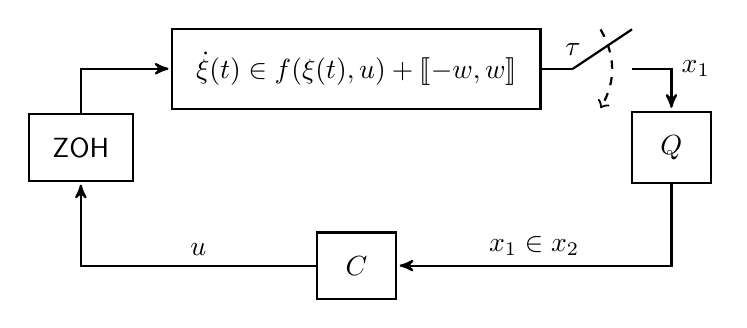
\begin{tikzpicture}
    [
    mynode/.style={draw,
                   thick,
                   inner sep=.3cm,
                   minimum width=1cm},
    %
    to/.style={->,
               >=stealth',
               shorten >=1pt,
               thick},
    ]

    \node [mynode] (sys) at (0,0) {$\dot \xi(t)\in f(\xi(t),u)+\segcc{-w,w}$};
    \node [mynode] (con) at (0,-2.5) {$C$};
    \node [mynode] (zoh) at (-3.5,-1) {$\mathsf{ZOH}$};

    %\node [mynode] (dist) at (4,0) {$P$};
    \node [mynode] (quant) at (4,-1) {$Q$};

    \node at (2.75,0.25) {$\tau$};


    \draw [to]  (zoh.north) |-  (sys.west);
    \draw [to]  (con.west)  -| node[above, near start] {$u$} (zoh.south);

    \draw[to] (3.5,0) -| node[right] {$x_1$} (quant.north);
    \draw[to] (quant.south) |- node[above, near end] {$x_1\in x_2$} (con.east);

    \draw[thick] (sys.east) -- (2.75,0);
    \draw[thick] (2.75,0) -- (3.5,.5);
    \draw[dashed,thick,bend left,->] (3.1,.5) to (3.1,-.5);

  \end{tikzpicture}
\caption{Sample-and-hold implementation of a controller synthesized with {\tt SCOTS}.}\label{f:closedloop}
\end{figure}

%In case that
%$\Sigma_1$ is an invariance or a reachability specification, the solution $C$ is
%a \emph{static} system, which means that the state alphabet is a singleton, i.e.,
%$X_c=\{x_c\}$. The output function 
%
%In the simplest
%case, $C$ is a \emph{static} system, which means $X_c$

Additionally to the perturbations on the right-hand-side
of~\eqref{e:sys:ct}, it is possible to account for measurement errors
modeled by a set-valued map $P \colon \mathbb{R}^n \rightrightarrows
\mathbb{R}^n$ given by
\begin{IEEEeqnarray}{c't'c}\label{e:theory:perturbation}
  P(x):=x+\segcc{-z,z} & with & z\in\R_+^n.
\end{IEEEeqnarray}
Please see~\cite[Sec.~VI.B]{ReissigWeberRungger15} and~\cite{RunggerZamani16}
for some background theory.
The closed loop with measurement errors is illustrated
in~Fig.~\ref{f:closedloop:pert}.
\begin{figure}[h]
\centering
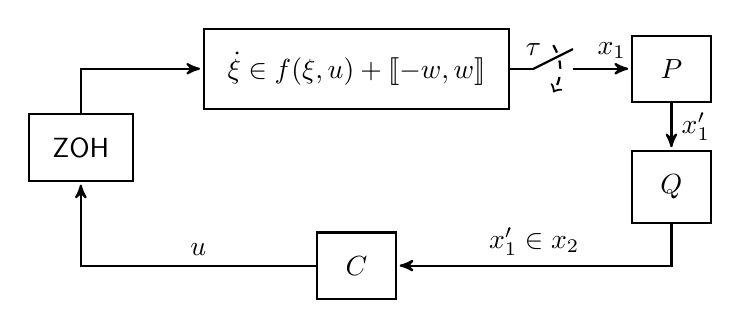
\begin{tikzpicture}
  [
  mynode/.style={draw,
                 thick,
                 inner sep=.3cm,
                 minimum width=1cm},
  %
  to/.style={->,
             >=stealth',
             shorten >=1pt,
             thick},
  ]

  \node [mynode] (sys) at (0,0) {$\dot \xi\in f(\xi,u)+\segcc{-w,w}$};
  \node [mynode] (con) at (0,-2.5) {$C$};

  \node [mynode] (zoh) at (-3.5,-1) {$\mathsf{ZOH}$};

  \node [mynode] (dist) at (4,0) {$P$};
  \node [mynode] (quant) at (4,-1.5) {$Q$};

  \node at (2.25,0.25) {$\tau$};


  \draw[thick] (sys.east) -- (2.25,0);
  \draw[thick] (2.25,0) -- (2.75,.25);
  \draw[dashed,thick,bend left,->] (2.5,.3) to (2.5,-.3);
  \draw[thick] (2.75,0) -- (3,0);

  \draw[to] (3,0) -- node[above] {$x_1$} (dist.west);
  \draw[to] (dist.south) -- node[right] {$x_1'$} (quant.north);


  \draw [to]  (zoh.north) |-  (sys.west);
  \draw [to]  (con.west)  -| node[above, near start] {$u$} (zoh.south);

  \draw[to] (quant.south) |- node[above, near end] {$x'_1\in x_2$} (con.east);

\end{tikzpicture}
\caption{Closed loop with measurement errors modeled by the set-valued map $x'_1 \in P(x_1)$.}\label{f:closedloop:pert}
\end{figure}

\section{Construction of Symbolic Models}

\subsection{Growth Bound and A Priori Enclosure}
\label{ss:GB} 

The construction of a symbolic model $S_2$ of $S_1$
is based on the over-approxima\-tion of
attainable sets. In {\tt SCOTS}, the over-approximation of the attainable sets
requires a so-called growth bound~\cite{ReissigWeberRungger15}.
A \emph{growth bound} of~\eqref{e:sys:ct} is a function $\beta \colon
\mathbb{R}_{+}^n \times U' \to \mathbb{R}_{+}^n$, which is defined with respect to a sampling time
$\tau>0$, a set $K\subseteq \mathbb{R}^n$ and a set $U'\subseteq U$.
Basically, it provides an upper bound on the deviation of solutions $\xi$
of~\eqref{e:sys:ct} from \emph{nominal
solutions}\footnote{A nominal solution $\varphi(\cdot,p,u)$ of
\eqref{e:sys:ct} is defined as solution of the initial value problem $\dot x=f(x,u)$,
$x(0)=p$.} $\varphi$ of~\eqref{e:sys:ct}, i.e., for every solution $\xi$ of
\eqref{e:sys:ct} on $\intcc{0,\tau}$ with input $u \in U'$ and $\xi(0)$, $p \in K$
we have
\begin{IEEEeqnarray}{c}
\label{e:growthbound}
| \xi(\tau) - \varphi(\tau,p,u) | \leq \beta( | \xi(0) - p |, u).
\end{IEEEeqnarray}
Here, $|x|$ for $x\in\R^n$, denotes the component-wise absolute value.
Essentially, a growth bound can be obtained by bounding
the Jacobian of $f$. Let
$L \colon U' \to \mathbb{R}^{n \times n}$ satisfy
\begin{IEEEeqnarray}{c}\label{e:theory:lipschitz}
L_{i,j}(u)
\geq
\begin{cases}
D_j f_i(x,u)& \text{if $i=j$,}\\
| D_j f_i(x,u) |& \text{otherwise}
\end{cases}
\end{IEEEeqnarray}
for all $x\in K'\subseteq \R^n$ and $u\in U'\subseteq U$. Then 
\begin{IEEEeqnarray}{c}
\label{e:GrowthBoundComputation}
\beta(r,u)
=
e^{L(u)\tau}
r
+
\int_0^\tau
e^{L(u)s}
w
\;\mathrm{d}s,
\end{IEEEeqnarray}
is a growth bound on $\intcc{0,\tau}$, $K$, $U'$
associated with \eqref{e:sys:ct}. The set $K'$ on
which~\eqref{e:theory:lipschitz} needs to hold, is a so-called \emph{a priori
enclosure}, i.e., $K'$  is assumed to be convex and contain any
solution $\xi$ on $\intcc{0,\tau}$ of~\eqref{e:sys:ct} with $u\in U'$ and
$\xi(0)\in K$,
see~\cite[Thm.~VIII.5]{ReissigWeberRungger15}. 

In order to use {\tt SCOTS}, the user needs to provide a growth bound, which for
nonlinear control systems can be provided in terms of the parameterized matrix
$L(u)$ whose entries satisfy~\eqref{e:theory:lipschitz}. A priori enclosures as well
as growth bounds can be computed automatically using interval arithmetic based
ODE solvers. See Section~\ref{s:usage:abs} for more details on how to
automatically obtain a priori enclosures and growth bounds.
%An implementation of such computations using the interval ODE
%solver {\tt vnode-lp} for the aircraft example can be found in the directory
%\begin{lstlisting}[basicstyle=\small\ttfamily]
%./examples/aircraft/helper        	
%\end{lstlisting}


\subsection{The Transition Function}
\label{s:theory:tf}

Recall that the state alphabet $X_2$ of the symbolic model \eqref{e:abs:sys} is composed of the real quantizer symbols $\bar X_2$, which are cells aligned on a
uniform grid, and the overflow symbols $X_2\smallsetminus \bar X_2$. For $x_2\in
X_2\smallsetminus \bar X_2$ the transition function is defined for all $u\in
U_2$ by
\begin{IEEEeqnarray}{c}\label{e:theory:tf1}
  F_2(x_2,u):=\emptyset.
\end{IEEEeqnarray}
In order to determine the successors $x_2'\in F_2(x_2,u)$ for 
$x_2=c+\segcc{-\eta/2,\eta/2}\in \bar X_2$ and $u\in U_2$, we first compute the
hyper-interval 
\begin{IEEEeqnarray}{c}\label{e:theory:attainableset}
  R:=\varphi(\tau,c,u)+\segcc{-\beta(\eta/2,u),\beta(\eta/2,u)}
\end{IEEEeqnarray}
which is an over-approximation of the attainable set of~\eqref{e:sys:ct}
with respect to the set $c+\segcc{-\eta/2,\eta/2}$ and input $u$.
If $P$ is not covered by the real quantizer symbols, i.e.,  $R\not\subseteq
\cup_{x_2\in \bar X_2} x_2$, then we define
\begin{IEEEeqnarray}{c}
  F_2(x_2,u):=\emptyset.
\end{IEEEeqnarray}
Otherwise, we define the successor cells function by
\begin{IEEEeqnarray}{c}\label{e:theory:tf3}
x_2'\in F_2(x_2,u):\iff x_2'\cap R\neq\emptyset.
\end{IEEEeqnarray}
Using similar arguments as in~\cite[Thm.~VIII.4]{ReissigWeberRungger15}, it is
straightforward to show that $Q$ is a feedback refinement relation from $S_1$ to
$S_2$. Note that $F_2$ satisfies 
\begin{IEEEeqnarray}{c}\label{e:theory:tf4}
 F_2(x_2,u)\subseteq \bar X_2.
\end{IEEEeqnarray}

If we need to be robust against measurement errors $P(x)=x+\segcc{-z,z}$, we
slightly modify the computation of $R$ to 
\begin{IEEEeqnarray}{c}
  R:=\varphi(\tau,c,u)+\segcc{-\beta(\eta/2+z,u),\beta(\eta/2+z,u)}
\end{IEEEeqnarray}
and define the transition function to (instead of~\eqref{e:theory:tf3})
\begin{IEEEeqnarray}{c}
x_2'\in F_2(x_2,u):\iff (x_2'+\segcc{-z,z})\cap R\neq\emptyset.
\end{IEEEeqnarray}
As a result we obtain that $Q\circ P$ is a feedback refinement relation from
$S_1$ to $S_2$, see~\cite[Thm.~III.5]{WeberRunggerReissig17}, which enables the
correct controller refinement under measurement errors~\cite[Sec.~VI.B]{ReissigWeberRungger15}. The use of the
perturbation parameter $z\in\R_{>0}^n$ in {\tt SCOTS} is explained in detail in 
Section~\ref{s:usage:abs}.

In the implementation of the computation of $F_2$ in {\tt Abstraction.hh}, we use a numerical ODE solver to compute an approximation of $\varphi(\tau,c,u)$ as well as $\beta(\eta/2,u)$.

\section{Controller Synthesis}
\label{s:theory:alg}

In this section, we discuss the algorithms that are implemented in {\tt SCOTS} to
solve synthesis problems for the finite symbolic model \eqref{e:abs:sys}. 
Usually, synthesis algorithms are developed in the context of two-player games on graphs. The player associated with the controller tries to
enforce the specification while the player associated with disturbances tries to
violate the specification, e.g.~\cite{BloemJobstmannPitermanPnueliSaar12}.

Given a control problem $(S_2,\Sigma_2)$ with $S_2$ given in~\eqref{e:abs:sys},
the construction of a controller to enforce a specification $\Sigma_2$ proceeds in two
steps. First, a subset $Y_\infty$ of the state alphabet $X_2$ is computed, which
characterizes the largest set of initial states so that the control problem is
solvable, i.e., $(S_2,\Sigma_2)$ is solvable if and only if $X_{2,0}\subseteq
Y_\infty$. The set $Y_\infty$ is referred to as \emph{winning domain} (or set of \emph{winning
states}) associated with $(S_2,\Sigma_2)$.
In a second step, the controller $C$ is derived form the set $Y_\infty$ and some other information available in synthesis algorithm.

We use the following notation. The set of \emph{admissible inputs} at $x_2\in X_2$ is denoted by
\begin{IEEEeqnarray}{c}
U_{S_2}(x_2):=\{u\in U_2\mid F_2(x_2,u)\neq\emptyset\}.
\end{IEEEeqnarray}
We use the Weierstrass symbol $\wp$ to denote the power set and define $\pre:\wp(X_2)\to \wp(X_2)$ by
\begin{IEEEeqnarray}{c}\label{e:pre}
  \pre(Y):=\{x_2\in X_2\mid  \exists_{u\in U_{S_2}(x_2)}:\;F_2(x_2,u)\subseteq Y\}.
\end{IEEEeqnarray}

\subsection{Invariance}

Let $\Sigma_2$ be an invariance specification associated with $Z_2$. 
We use Alg.~\ref{a:safety}, which is implemented in the function {\tt solve\_invariance\_game} in the file {\tt GameSolver.hh}, to synthesize a controller
that solves the control problem $(S_2,\Sigma_2)$.  
Alg.~\ref{a:safety} runs in $O(m)$ time, where $m$ is the number of transitions, i.e., the number of
triples $(x_2,u,x'_2)$ with $x'_2\in F_2(x_2,u)$, since each state is added to the queue
of bad states $Q$ at most once.

\begin{algorithm}[h]
\caption{Controller synthesis for invariance specs associated  $Z_2$}\label{a:safety}
  \begin{algorithmic}[1]
    \Input{$Z_2$, $S_2=(X_2,U_2,F_2)$}
    \Require{$F_2(X_2,U_2)\subseteq \bar X_2$ and $Z_2\subseteq \bar X_2$}
    \State $Q:=\emptyset$ \Comment{ FIFO queue of bad states} 
    \State $E:=\emptyset$ \Comment{ bookkeeping of the bad states} 
    \State $D:=\emptyset$ \Comment{ valid state-input pairs}
    \ForAll{$x_2\in \bar X_2$}
    \If{$x_2\not\in Z_2$ or $U_2(x_2)=\emptyset$}
    \Comment{ mark all states outside $Z_2$ or blocking states as bad}
    \State $Q:=Q\cup \{x_2\}$
    \Else 
    \State $D:=D\cup (\{x_2\}\times U_2(x_2))$ 
    \EndIf
    \EndFor
    \State $E:=Q$
    \While{ $Q\neq\emptyset$ }
    \State $x'_2:\in Q$ \Comment{remove oldest element}\label{a:safety:beginwhile}
    \State $Q:=Q\smallsetminus \{x_2'\}$\label{a:safety:remQ}
    \ForAll{$(x_2,u)\in F_2^{-1}(x_2')$}
    \State $D:=D\smallsetminus \{(x_2,u)\}$\label{a:safety:remove}
    \Comment{ remove state-input pairs that lead to bad states}
    \If{$x_2\not \in D^{-1}(U_2)$ and $x_2\not\in E$}
    \Comment{ no valid input left and not already marked bad}
    \State $Q:=Q\cup\{x_2\}$\label{a:safety:addQ}
    \Comment{ add to queue of bad states}
    \State $E:=E\cup\{x_2\}$\label{a:safety:addE}
    \EndIf
    \EndFor
    \EndWhile
    \Output $D$
  \end{algorithmic}

\end{algorithm}

Let $D\subseteq X_2\times U_2$ be the set of state-input pairs computed in
Alg.~\ref{a:safety}. One can show that $D^{-1}(U_2)$ is the \emph{maximal fixed
point} of the map $G:\wp(X_2)\to \wp(X_2)$ defined by
\begin{IEEEeqnarray}{c}\label{e:theory:fp:safety}
  G(Y):=Z_2\cap\pre(Y).
\end{IEEEeqnarray}
The maximal fixed point of~\eqref{e:theory:fp:safety} corresponds to the winning domain
of $(S_2,\Sigma_2)$ and it follows that the synthesis problem $(S_2,\Sigma_2)$ is solvable if and only
if $X_{2,0}\subseteq D^{-1}(U_2)$. 

%\begin{lemma}
%Let $S_2=(X_2,U_2,F_2)$ be a finite simple system with $\bar X_2\subseteq X_2$
%and $F_2(X_2,U_2)\subseteq \bar X_2$. Let $Z_2\subseteq \bar X_2$ and let $D$ be the output of
%Alg.~\ref{a:safety}. The set $Y_\infty:=D^{-1}(U_2)$ is the maximal fixed point
%of~\eqref{e:theory:fp:safety}.
%\end{lemma}
%\begin{proof}
%Let $D_i$, $E_i$ and $Q_i$ denote the sets $D$, $E$ and $Q$
%manipulated in Alg.~\ref{a:safety} at the beginning of the while loop in
%line~\ref{a:safety:beginwhile} of iteration $i\in \Z_{\ge0}$. For example for
%$i=0$ we have $D_0=\{(x,u) \mid x\in Z_2\wedge u\in U_{S_2}(x)\}$ and $D_{i+1}$
%results from $D_i$ by removing the elements in line~\ref{a:safety:remove}.
%Similarly, $E_0=Q_0$ and $E_{i+1}$ results from $E_i$ by adding elements in
%line~\ref{a:safety:addE} and $Q_{i+1}$ results from $Q_i$ by adding and removing
%elements in line~\ref{a:safety:addQ} and line~\ref{a:safety:remQ}, respectively.
%Parallel to $D_i$ we introduce $Y_i:=D_i^{-1}(U_2)$.  Let us point out that for
%all $i\ge0$ we have $Q_i\subseteq E_i$, $E_i=\cup_{i'\in\intcc{0;i}} Q_{i'}$ and the sets 
%$E_i$ and $Y_i$ are disjoint and satisfy $\bar X_2=E_i\cup Y_i$. Also $Y_{i+1}\subseteq Y_i\subseteq \cdots
%\subseteq Z_2$ and there exists $i^*\in \Z_{\ge0}$ so that $Y_{i^*}=Y_\infty$.
%
%Let us first show that $Y_\infty=G(Y_\infty)$. Let $Y_\infty
%=Y_{i^*}$ and $x\in Y_{i^*}$. Since $Y_{i^*}\subseteq Z_2$ we have $x\in Z_2$
%and it remains to show that $x\in \pre(Y_{i^*})$. Let
%$u\in U_{S_2}(x)$ be such that $(x,u)\in D_{i^*}$. As $(x,u)\in D_{i^*}$ we
%conclude $F(x,u)\cap Q_i=\emptyset$ for all $i\in\intcc{0;i^*}$ (otherwise
%$(x,u)$ would have been removed in line~\ref{a:safety:remove}). We obtain
%$F(x,u)\cap E_{i^*}=\emptyset$. Since $F_2(x,u)\subseteq \bar X_2$ and $\bar
%X_2=E_{i^*}\cup Y_{i^*}$ it follows that $F_2(x,u)\subseteq Y_{i^*}$ and $x\in
%\pre(Y_{i^*})$ follows.  Now let $x\in G(Y_{i^*})=Z_2\cap \pre(Y_{i^*})$ and
%assume for the sake of contradiction that $x\not\in Y_{i^*}$.
%Let $u\in U_{S_2}(x)$ so that $F_2(x,u)\subseteq Y_{i^*}$. Since
% $x\in Z_2$ we see that $(x,u)\in D_0$. Hence, if $x\not\in Y_{i^*}$ all pairs $(\bar x,\bar u)$
%with $\bar x=x$ (including the pair $(x,u)$) need to have been removed from $D_0$ along the iteration
%$i\in\intcc{0;i^*}$. However, from $F_2(x,u)\subseteq Y_{i^*}$ follows that
%$F_2(x,u)\cap E_{i^*}=\emptyset$. Moreover, 
%for all $i\in\intcc{0;i^*}$ holds $Q_i\subseteq E_{i^*}$ and we obtain $F_2(x,u)\cap
%  Q_{i}=\emptyset$ for all $i\in\intcc{0;i^*}$ so that we arrive at a contradiction
%  since $(x,u)$ cannot have been removed from $D_0$ in line~\ref{a:safety:remove}.
%
%Let $\bar Y\subseteq X_2$. We show that $\bar Y \subseteq G(\bar Y)$ implies
%$\bar Y\subseteq Y_\infty$ by induction over  $i\ge 0$.
%Let $i=0$ and $x\in \bar Y$. Since
%$\bar Y\subseteq G(\bar Y)$ we have $x\in Z_2$ and $U_{S_2}(x)\neq\emptyset$,
%which shows that $x\in Y_0$. Now suppose that $\bar Y\subseteq Y_i$ but $\bar
%Y\not\subseteq Y_{i+1}$, i.e., there exist $x\in (Y_i\smallsetminus Y_{i+1})\cap
%\bar Y$. That means all pairs $(\bar x,\bar u)$ with $\bar x=x$ in $D_i$ have been removed in line~\ref{a:safety:remove}. 
%However, there exists at least one $u\in U_{S_2(x)}$ with
%$F_2(x, u)\cap Q_i=\emptyset$. That follows from
%the fact that $x\in G(\bar Y)$, $\bar Y\subseteq Y_i$ and $Q_i\cap Y_i\neq
%\emptyset$. Hence,
%we obtain a contradiction and $\bar Y\subseteq Y_{i+1}$ follows. As this holds
%for all $i\ge0$ we conclude that $\bar Y\subseteq Y_{\infty}$ and the assertion follows.
%\end{proof}


Suppose that $X_{2,0}\subseteq D^{-1}(U_2)$ holds, then we obtain a controller
$C=(\{q\},\{q\},X_2,X_2,U_2,F_c,H_c)$
that solves $(S_2,\Sigma_2)$ by  
\begin{IEEEeqnarray}{rCl}\label{e:theory:controller}
\begin{IEEEeqnarraybox}[][c]{rCl}
H_c(q,x_2)&=&
\begin{cases}
D(x_2)\times \{x_2\} & \text{if } x_2\in D^{-1}(U_2)\\
U_2\times\{x_2\} & \text{otherwise}
\end{cases}\\
F_c(q,x_2)&=&
\begin{cases}
\{q\} & \text{if } x_2\in D^{-1}(U_2)\\
\emptyset &  \text{otherwise.}
\end{cases}
\end{IEEEeqnarraybox}
\end{IEEEeqnarray}
The refined controller that solves $(S_1,\Sigma_1)$ is given by $C\circ Q$.
Note that the definition of the initial state alphabet $X_{2,0}$
in~\eqref{e:theory:abs:initial} and the condition $X_{2,0}\subseteq
D^{-1}(U_2)$ imply that the initial state alphabet of $S_1$ satisfies
\begin{IEEEeqnarray}{c}\label{e:theory:refinement:initial}
X_{1,0}\subseteq \cup_{x_2\in D^{-1}(U_2)} x_2. 
\end{IEEEeqnarray}
The controller $C\circ Q$ is implemented in {\tt SCOTS} in the {\tt StaticController} class. 
The details are
explained in Section~\ref{s:usage:simulation}.


\subsection{Reachability}

Let $\Sigma_2$ be a reachability specification associated with
$Z_2\subseteq \bar X_2$. 
We use Alg.~\ref{a:reach}, which is implemented in the function 
{\tt solve\_reachability\_game} in the file {\tt GameSolver.hh}, to synthesize a controller
that solves the control problem $(S_2,\Sigma_2)$. The algorithm is a variant of
Dijkstra's shortest path algorithm for hyper-graphs taken
from~\cite{GalloLongoPallotinoNguyen93}. It runs in $O(m)$ time, where $m$ is
the number of transitions, i.e., the number of elements in $X_2\times U_2\times
X_2$ that satisfy $x_2'\in F_2(x_2,u)$.

\begin{algorithm}[h]
  \caption{Controller synthesis for reachability specs associated with $Z_2$}
  \label{a:reach}
  \begin{algorithmic}[1]
    \Input{ $Z_2$, $S_2=(X_2,U_2,F_2)$, $u_0\in U_2$}
    \Require{ $Z_2\subseteq \bar X_2$}
    \State {$Q := Z_2$ \Comment{FIFO queue}}
    \State {$V := \infty$}\Comment{value function}\label{a:reach:initV}
    \State $M:=0$ \Comment{intermediate values} 
    \State {$E := \emptyset$ \Comment{bookkeeping of processed states}}
    \ForAll {$x_2 \in\bar X_2$}
      \State {$D(x_2) := \emptyset$}\Comment{keep track of optimal input}
      \If{$x_2\in Z_2$}
        \State {$V(x_2) := 0$}\Comment{cost at target are zero}
        \label{a:reach:setV}
        \State {$D(x_2) := \{u_0\}$}\label{a:reach:initD}
        \label{a:reach:initD}
      \EndIf
    \EndFor
    \While {$Q \not= \emptyset$}
      \State {$x_2' :\in  Q $} \Comment{remove oldest element} \label{a:reach:remove}
      \State {$Q := Q \smallsetminus \{ x_2' \}$}
      \State {$E := E \cup \{ x_2' \}$}\label{a:reach:addE}
      \ForAll {$(x_2,u) \in F_2^{-1}(x_2')$}
        \State $M(x_2,u):=\max\{M(x_2,u),V(x_2')\}$
        \If {$F_2(x_2,u) \subseteq E$ and $V(x_2) > 1+M(x_2,u)$} \Comment{if $u$ leads to better cost update input}
        \label{a:reach:conditions}
          \State {$V(x_2) := 1+M(x_2,u)$} \label{a:reach:updateV}
          \State {$Q := Q \cup \{ x_2 \}$}\label{a:reach:add}
          \State {$D(x_2) := \{ u \}$}\label{a:reach:setD}
        \EndIf
      \EndFor
    \EndWhile
    \Output {$D$, $V$}
  \end{algorithmic}
\end{algorithm}

Let $D$ be the output of Alg.~\ref{a:reach}.
The set $D^{-1}(U_2)$ is
the \emph{minimal fixed point} of the map $G:\wp(X_2)\to \wp(X_2)$ defined by
\begin{IEEEeqnarray}{c}\label{e:theory:fp:reach}
  G(Y):=Z_2\cup\pre(Y).
\end{IEEEeqnarray}
The minimal fixed point of~\eqref{e:theory:fp:reach} corresponds to the winning
domain of $(S_2,\Sigma_2)$ and it follows that the synthesis problem $(S_2,\Sigma_2)$ is solvable if and only
if $X_{2,0}\subseteq D^{-1}(U_2)$. 

%\begin{lemma}
%Let $S_2=(X_2,U_2,F_2)$ be a finite simple system with $\bar X_2\subseteq X_2$,
%let $Z_2\subseteq \bar X_2$  and let $D$ be the output of
%Alg.~\ref{a:reach}. Then $Y_\infty:=D^{-1}(U_2)$ is the minimal fixed point
%of~\eqref{e:theory:fp:reach}.
%\end{lemma}
%\begin{proof}[Proof sketch]
%Let $Q_i$ denote the set $Q$ that is processed Alg.~\ref{a:reach} at iteration
%$i$ of the while loop in line~\ref{a:reach:remove}. For example $Q_0=Z_2$ and
%$Q_{i+1}$ results from $Q_i$ by removing and adding elements in
%line~\ref{a:reach:remove} and~\ref{a:reach:add}, respectively. Let $i^*$ denote
%the iteration when the algorithm terminates, i.e., $Q_{i^*}=\emptyset$. Since
%every element of $Q_i$ for all $i\in\intco{0;i^*}$ is added to $E$ in
%line~\ref{a:reach:addE}, we have 
%$E=\cup_{i\in\intcc{0;i^*}}Q_i$. Moreover, $D(x)\neq\emptyset$ holds iff 
%$x\in Q_i$ for some $i\in\intco{0;i^*}$ and we see that $Y_\infty=E$.
%Another invariant which is easy to check is: $x\in Q_i$ for some $i\in
%\intco{0;i^*}$ implies $V(x)<\infty$. Hence $M(x,u)$ is finite for every
%$(x,u)\in X_2\times U_2$ throughout the whole computation.
%
%Let us show that $Y_\infty$ is a fixed point of~\eqref{e:theory:fp:reach}.
%Let $x\in Y_\infty$. If $x\in Z_2$ we immediately obtain $x\in G(Y_\infty)$.
%For $x\not\in Z_2$ we see that $D(x)$ has been set in line~\ref{a:reach:setD}
%and we obtain $F_2(x,D(x))\subseteq E=Y_\infty$. Now let $x\in G(Y_\infty)$. If
%$x\in Z_2$ we use line~\ref{a:reach:initD} to infer $x\in Y_\infty$ and
%subsequently we consider $x\in \pre(Y_\infty)$. Since $Y_\infty=E$, there exists
%$u\in U_{S_2}(x)$ so that $F_2(x,u)\subseteq E$. Since $M(x,u)<\infty$ holds
%throughout the computation and initially $V(x)=\infty$, we see that there must have been an iteration $i$ where
%both conditions in line~\ref{a:reach:conditions} have been true for $(x,u)$ (in
%place of $(x_2,u)$), so that
%$D(x)\neq\emptyset$, which shows $x\in Y_\infty$.
%
%We continue to show that $Y_\infty$ is the minimal fixed point
%of~\eqref{e:theory:fp:reach}.
%Let $D_i$ denote the map $D$ computed in Alg.~\ref{a:reach} at
%line~\ref{a:reach:remove}, i.e., $D_0$ is
%computed in line~\ref{a:reach:initD} and $D_{i+1}$ results from $D_i$ by setting
%the input in line~\ref{a:reach:setD}. Let $Y_i:=D_i^{-1}(U_2)$ and observe that
%$Y_0=Z_2$ and $Y_i\subseteq Y_{i+1}$ holds for all $i\ge0$. One can also show
%that $Y_{i+1}\subseteq G(Y_i)$.
%Moreover, one can show that $G$ is monotone, i.e., for  $Y,Y'\subseteq \bar X_2$ the inclusion
%$Y\subseteq Y'$ implies $G(Y)\subseteq G(Y')$. Given this fact it is easy to see
%that $G(\bar Y)\subseteq \bar Y$ implies $Y_{i}\subseteq \bar Y$ for all $i\ge0$, since we
%have $Y_0=Z_2\subseteq \bar Y$ and $Y_{i+1}\subseteq G(Y_i)\subseteq G(\bar
%Y)\subseteq \bar Y$. Given that the algorithm terminates there exists $i^*$ with
%$Y_\infty=Y_{i^*}$ and $Y_\infty\subseteq \bar Y$ follows.
%\end{proof}

Given that $X_{2,0}\subseteq D^{-1}(U_2)$ holds, a controller
$C=(\{q\},\{q\},X_2,X_2,U_2,F_c,H_c)$ that solves $(S_2,\Sigma_2)$ is identical
to the controller that solves the invariance problem, i.e., $F_c$ and $H_c$ are
given by~\eqref{e:theory:controller}.

Again, the refined controller $C\circ Q$ that is feedback composed with $S_1$ is
implemented in {\tt SCOTS} in the {\tt StaticController} class. The details are
explained in Section~\ref{s:usage:simulation}.

\subsection{Reach-Avoid}
Let $\Sigma_2$ be a reach-avoid specification associated with $A_2$, $Z_2\subseteq \bar X_2$. 
{\tt SCOTS} provides two alternatives to synthesize controllers to enforce
reach-avoid specifications. In the first method, the avoid set $A_2$ is
accounted for in the transition function, i.e.,
\begin{IEEEeqnarray}{c'c}\label{e:theory:tf:avoid}
  \forall_{x_2\in A_2}:& F_2(x_2,u):=\emptyset.
\end{IEEEeqnarray}
In this way we can reduce a reach-avoid problem to a reachability problem. 
Given that the transition function satisfies \eqref{e:theory:tf:avoid}, any
controller that solves the control problem $(S_2,\Sigma_2')$, where $\Sigma_2'$
is the reachability specification associated with $Z_2$, also solves the
control problem $(S_2,\Sigma_2)$. In order to enforce the
equation~\eqref{e:theory:tf:avoid} in the computation of the transition function
$F_2$ the user can optionally supply the avoid set to the function {\tt
Abstraction::compute\_gb}, see Section~\ref{s:usage:abs}.

For the second method, the computation of the transition function is left
unchanged, but Alg.~\ref{a:reach} is modified to account for the avoid set. To
this end the condition in line~\ref{a:reach:conditions} in Alg.~\ref{a:reach} is modified to 
\begin{IEEEeqnarray}{c't'c't'c}\label{a:avoid}
 F_2(x_2,u) \subseteq E& and &V(x_2) > 1+M(x_2,u)& and & x_2\not\in A_2.
\end{IEEEeqnarray}
Again the user can optionally supply the avoid set to the function {\tt
solve\_reachability\_game}, see Section~\ref{s:usage:synthesis}.


%\subsection{Customized Synthesis Algorithms}
%\label{s:theory:customized}
%
%Even though {\tt SCOTS} natively supports only invariance and reachability
%specification, an advanced user has the possibility to write customized
%synthesis algorithms. We demonstrate such a customization for persistence and
%recurrence specifications. 
%
%Let $S=(X,U,F)$ be a finite simple
%system with and consider the sets $I, Z, T_i\subseteq X$, $i\in\intcc{1;p}$,
%$p\in\N$. The \emph{persistence} specification $\Sigma$ for $S$ associated with $I$ and $Z$ is given by
%\begin{IEEEeqnarray}{c}
%  \Sigma:=\big\{(u,x)\in (U\times X)^\infty
%  \mid  x(0)\in I\implies 
%    \exists_{t\in\intco{0;\infty}}\forall_{t'\in\intcc{t;\infty}}: x(t')\in Z
%  \big\}.
%\end{IEEEeqnarray}
%The \emph{recurrence} specification $\Sigma$ for $S$ associated with $I$ and
%$T_i$, $i\in\intcc{1;p}$, $p\in\N$ is given by
%\begin{IEEEeqnarray}{c}
%  \Sigma:=\big\{(u,x)\in (U\times X)^\infty
%  \mid  x(0)\in I\implies 
%    \forall_{t\in\intco{0;\infty}}\forall_{i\in\intcc{1;p}}\exists_{t'\in\intcc{t;\infty}}:
%    x(t')\in T_i
%  \big\}.
%\end{IEEEeqnarray}
%Using the $\mu$-calculus notation, e.g. used
%in~\cite{BloemJobstmannPitermanPnueliSaar12}, to denote minimal and maximal fixed
%points of monotone functions, we can characterize the set of \emph{winning
%states} for persistence and recurrence specifications by the fixed point expressions
%\begin{IEEEeqnarray}{c}
%  \mu Y_1.\nu Y_2. \pre(Y_1)\cup (\pre(Y_2)\cap Z)
%\end{IEEEeqnarray}
%respectively
%\begin{IEEEeqnarray}{c}
%  \nu Y_1.\bigcap_{i\in\intcc{1;p}}\mu Y_2. \pre(Y_2)\cup (\pre(Y_1)\cap T_i).
%\end{IEEEeqnarray}


\newpage


\part{USAGE}

\section{Computation of Symbolic Models}
\label{s:usage:abs}

Let $S_1$ be a simple system that represents the $\tau$-sampled
behavior of the continuous-time system~\eqref{e:sys:ct} as defined in~\eqref{e:sys}.
In order to compute the transition function $F_2$ of a symbolic
model~\eqref{e:abs:sys} of $S_1$ in {\tt SCOTS}, the following ingredients are
needed.
\begin{enumerate}
  \item The solution $\varphi(\tau,x,u)$ of the IVP $\dot \xi = f(\xi,u)$,
  $\xi(0)=x$ at time $\tau$, which is provided in terms of a lambda expression
  of the form 
\begin{lstlisting}[basicstyle=\small\ttfamily, language=C++]
[](state_type& x, const input_type& u)  -> void {}
\end{lstlisting}
  The state solution of the IVP at time $\tau$, i.e., $\varphi(\tau,x,u)$ is
  expected to be stored in the variable~{\tt x}. The {\tt state\_type} and
  {\tt\small input\_type} are aliases for {\tt\small std::array<double,dim>} in the appropriate
  dimension.

  \item A growth bound $\beta(r,u)$, which is provided by a lambda expression of
  the form
\begin{lstlisting}[basicstyle=\small\ttfamily, language=C++]
[](state_type& r, const state_type& c, const input_type& u)  -> void {}
\end{lstlisting}
  Again, the value of the growth bound $r'=\beta(r,u)$ is assumed to be stored
  in the variable {\tt r}. In the implementation, the growth bound is allowed
  to depend the center of the cell {\tt c}. See~\cite{WeberRunggerReissig17} for
  details.

  \item The set of real quantizer symbols $\bar X_2$ as defined
  in~\eqref{e:theory:ss}, which is defined as instantiation of the class with constructor
\begin{lstlisting}[basicstyle=\small\ttfamily, language=C++]
template<class grid_point_t>
scots::UniformGrid(const int dim,
                     const grid_point_t& lb,
                     const grid_point_t& ub,
                     const grid_point_t& eta)
\end{lstlisting}
  where the variables {\tt dim}, {\tt lb}, {\tt ub} and {\tt eta} represent the
  state space dimension, the lower and upper bound of the hyper-interval
  confining the set $\bar X_2$, and the grid parameter, respectively.

	Internally, each cell $x_2=c+\segcc{-\eta/2,\eta/2}\in\bar X_2$ is represented
  as an unsigned integer of type {\tt abs\_type}. In the default setting, {\tt
  abs\_type} is an alias set in {\tt UniformGrid.hh} to 
\begin{lstlisting}[basicstyle=\small\ttfamily, language=C++]
using abs_type=std::uint32_t;
\end{lstlisting}
  which limits the size of $\bar X_2$ to $2^{32}-1$. The template member functions 
\begin{lstlisting}[basicstyle=\small\ttfamily]
template<class grid_point_t>
scots::UniformGrid::itox(abs_type id, state_type& x)
template<class grid_point_t>
scots::UniformGrid::abs_type xtoi(const grid_point_t& x) const 
\end{lstlisting}
  are useful in mapping an abstract state $c+\segcc{-\eta/2,\eta/2}\in
  \bar X_2$, represented by its unsinged integer ID {\tt id}, to its center
  $c\in \R^n$ aligned on the uniform grid~\eqref{e:theory:grid}. Similarly, {\tt
  xtoi} can be used to map a state $x\in \R^n$ to the {\tt id} of the cell
  $x_2\in\bar X_2$ containing it, i.e., $x\in x_2$.

  \item The input alphabet $U_2$, which is again represented by an instance
  of a {\tt UniformGrid}.

  \item Optionally, it is possible to provide a measurement error bound to
  account for measurement errors as defined in~\eqref{e:theory:perturbation} using the
  member function
\begin{lstlisting}[basicstyle=\small\ttfamily]
scots::Abstraction::set_measurement_error_bound(const state_type& z)
\end{lstlisting}
\end{enumerate}

We demonstrate the usage of {\tt SCOTS} to compute a symbolic
model of the sampled dynamics of an aircraft used
in~\cite[Sec.~IX.B]{ReissigWeberRungger15}. The system consists of three states $x_1,x_2,x_3$, which respectively correspond to the velocity, the flight path angle and the altitude of the
aircraft. The input alphabet is given by $U =
\intcc{0,160\cdot 10^3} \times \intcc{0^\circ,10^\circ}$ 
and represents the thrust of the engines (in Newton) and the angle of attack.
Additionally, we use the disturbance vectors $w=(0.108,0.002,0)^\top$
in~\eqref{e:sys:ct} and  $z=(0.0125,0.0025^\circ,0.05)^\top$
in~\eqref{e:theory:perturbation} to model possible input
disturbances, respectively, measurement errors.

For the computation of the transition function, we begin with the aliases for the {\tt state\_type} and {\tt input\_type} by
\begin{lstlisting}[basicstyle=\small\ttfamily]
const int state_dim=3; /* state space dim */
const int input_dim=2; /* input space dim */
using state_type = std::array<double,state_dim>;
using input_type = std::array<double,input_dim>;
\end{lstlisting}
Afterwards, we define the lambda for the solution of the IVP for a
sampling time of $\tau=0.25$ by
\begin{lstlisting}[basicstyle=\small\ttfamily, language=C++]
auto aircraft_post = [](state_type &x, const input_type &u) {
  /* the ode describing the aircraft */
  auto rhs = [](state_type& xx,  const state_type &x, const input_type &u) {
    double mg = 60000.0*9.81;
    double mi = 1.0/60000;
    double c=(1.25+4.2*u[1]);
    xx[0] = mi*(u[0]*std::cos(u[1])-(2.7+3.08*c*c)*x[0]*x[0]-mg*std::sin(x[1]));
    xx[1] = (mi/x[0])*(u[0]*std::sin(u[1])+68.6*c*x[0]*x[0]-mg*std::cos(x[1]));
    xx[2] = x[0]*std::sin(x[1]);
  };
  /* use 10 intermediate steps */
  scots::runge_kutta_fixed4(rhs,x,u,state_dim,tau,10);
};
\end{lstlisting}
where we use the fixed step-size ODE solver {\tt scots::runge\_kutta\_fixed4} that
ships with {\tt SCOTS}. An implementation that uses a more advanced ODE solver like the
adaptive step-size solvers with error control implemented in {\tt boost} can be found in {\tt ./examples/aircraft\_boost}.

We continue with the definition of the growth bound, for which we determine the
matrix $L(u)$ in~\eqref{e:theory:lipschitz}. First, we compute an a priori
enclosure $K'$ of~\eqref{e:sys:ct} with respect to $\tau=0.25$, $U'=U$ and the
hyper-interval $P(K)$ where 
  $K=\intcc{58,83}\times\intcc{-3^\circ,0}\times \intcc{0,56}$
is the hyper-interval 
that confines the set of real quantizer symbols. To this end, we employ
the interval arithmetic based ODE solver implemented in
\href{http://www.cas.mcmaster.ca/~nedialk/vnodelp}{vnode-lp} to obtain 
\begin{IEEEeqnarray*}{c}
  K'=\intcc{57.55,83.23}\times\intcc{-4.29^\circ,1.22^\circ}\times \intcc{-1.38,56.28}.
\end{IEEEeqnarray*}
The implementation of the computation of the a priori enclosure can be found in
the example directory 
{\tt ./examples/aircraft/helper/a\_priori\_enclosure}.
To obtain the matrix $L(u)$, we maximize the partial derivatives of $f(\cdot,u)$ over the set $K'$. The solution of the linear IVP
$\dot r(t) = L(u) r(t)+ w$, $r(0)=r_0$, at time $\tau$
provides the growth bound \eqref{e:GrowthBoundComputation} that we access
through the lambda
\begin{lstlisting}[basicstyle=\small\ttfamily, language=C++]
auto radius_post = [](state_type &r, const state_type &, const input_type &u) {
  /* the ode for the growth bound */
  auto rhs =[](state_type& rr,  const state_type &r, const input_type &) {
    /* lipschitz matrix */
    double L[3][2];
    L[0][0]=-0.001919*(2.7+3.08*(1.25+4.2*u[1])*(1.25+4.2*u[1]));
    L[0][1]=9.81;
    L[1][0]=0.002933+0.004802*u[1];
    L[1][1]=0.00361225;
    L[2][0]=0.07483;
    L[2][1]=83.22;
    /* to account for input disturbances */
    state_type w={{0.108,0.002,0}};
    rr[0] = L[0][0]*r[0]+L[0][1]*r[1]+w[0]; 
    rr[1] = L[1][0]*r[0]+L[1][1]*r[1]+w[1]; 
    rr[2] = L[2][0]*r[0]+L[2][1]*r[1]+w[2]; 
  };
  /* use 10 intermediate steps */
  scots::runge_kutta_fixed4(rhs,r,u,state_dim,tau,10);
};
\end{lstlisting}
The real quantizer symbols $\bar X_2$ and the input
alphabet $U_2$ are introduced as instances of the class {\tt UniformGrid} by
\begin{lstlisting}[basicstyle=\small\ttfamily, language=C++]
  state_type s_lb={{58,-3*M_PI/180,0}};
  state_type s_ub={{83,0,56}}; 
  state_type s_eta={{25.0/362,3*M_PI/180/66,56.0/334}}; 
  scots::UniformGrid ss(state_dim,s_lb,s_ub,s_eta);

  input_type i_lb={{0,0}};
  input_type i_ub={{32000,8*M_PI/180}};
  input_type i_eta={{32000,8.0/9.0*M_PI/180}};
  scots::UniformGrid is(input_dim,i_lb,i_ub,i_eta);
\end{lstlisting}
The grid parameter {\tt\small s\_eta} for the real quantizer symbols $\bar X_2$
has been determined according to the optimization procedure
in~\cite{WeberRunggerReissig17}.

For the computation of the symbolic transition function $F_2$ we instantiate  the
class {\tt\small Abstraction} and set the measurement error bound to $z$
\begin{lstlisting}[basicstyle=\small\ttfamily, language=C++]
  scots::Abstraction<state_type,input_type> abs(ss,is);
  state_type z={{0.0125,0.0025/180*M_PI,0.05}};
  abs.set_measurement_error_bound(z);
\end{lstlisting}
The computation of $F_2$ itself is invoked by
\begin{lstlisting}[basicstyle=\small\ttfamily, language=C++]
  abs.compute_gb(tf,aircraft_post,radius_post);
\end{lstlisting}

Note that, due to the numerical errors in the computation of the solution of the
IVP $\varphi(\tau,x,u)$ it is possible that the computed transition function $F_2$ does not satisfies
the requirements in Sectin~\ref{s:theory:tf}. Similarly, the
computation of the growth bound $\beta(r,u)$ might be erroneous. 
Therefore, it is crucial to pick adequate ODE solver parameters to obtain 
high confidence in the correctness of the computation.

We list the runtimes of
the computation of $F_2$ for two different solvers for various parameters in
Table~\ref{t:runtimes:tf}. The implementations can be found in the directories
{\tt ./exampels/aircraft\_boost} and {\tt./examples/aircraft}.

\begin{table}[h]\label{t:runtimes:tf}
\begin{tabular}{C|C|C|C|C}
  \multicolumn{3}{c|}{adaptive step size {\tt runge\_kutta\_dopri5}} &
  \multicolumn{2}{c}{fixed step size {\tt runge\_kutta\_4} } \\
  \multicolumn{3}{c|}{{\tt abs\_tol/rel\_tol}} &
  \multicolumn{2}{c}{\# intermediate steps} \\
  $10^{-10}$/$10^{-10}$ & $10^{-12}$/$10^{-12}$& $10^{-16}$/$10^{-16}$ &  5 & 10\\\hline
  252$\;sec$ & 370$\;sec$ & 1036 $\;sec$ & 233 $\;sec$ & 335 $\;sec$
\end{tabular}
\caption{Runtimes to compute a symbolic transition function of the aircraft
dynamics  with varying ODE solvers and solver parameters. All computations
resulted in an identical transition function with $5.86\cdot10^9$ transitions.} 
\end{table}


\section{Controller Synthesis}
\label{s:usage:synthesis}

Let $\Sigma_2$ be an invariance or reachability specification associated with $Z_2\subseteq \bar
X_2$ for~\eqref{e:abs:sys}.
The algorithms Alg.~\ref{a:safety} and Alg.~\ref{a:reach} to compute the winning
domain $D^{-1}(U_2)$ associated with the control problem $(S_2,\Sigma_2)$
are implemented in the following functions.
\begin{enumerate}
  \item Alg.~\ref{a:safety} is implemented {\tt solve\_invariance\_game} with signature 
\begin{lstlisting}[basicstyle=\small\ttfamily]
template<class F> 
WinningDomain solve_reachability_game(const TransitionFunction& tf, F& ap)
\end{lstlisting}
  where the set $Z_2$ is defined as lambda expression {\tt ap} of the form
\begin{lstlisting}[basicstyle=\small\ttfamily]
[](const scots::abs_type& abs_state) -> bool {}
\end{lstlisting}
  {\tt ap(abs\_state)} returns {\tt true} if and only if the abstract state $x_2\in\bar X_2$, represented by
  the ID {\tt abs\_state}, is  an element of the safe set $Z_2$.

  \item Alg.~\ref{a:reach} is implemented in {\tt solve\_reachability\_game} with signature 
\begin{lstlisting}[basicstyle=\small\ttfamily]
template<class F>
WinningDomain solve_reachability_game(const TransitionFunction& tf, F& ap)
\end{lstlisting}
  where the target set $Z_2$ is defined as lambda expression {\tt ap} of the
  form
\begin{lstlisting}[basicstyle=\small\ttfamily]
[](const scots::abs_type& abs_state) -> bool {}
\end{lstlisting}
  {\tt ap(abs\_state)} returns {\tt true} if and only if the abstract state $x_2\in\bar X_2$, represented by
  the ID {\tt abs\_state}, is  an element of the safe set $Z_2$.

  \item Optionally, the IDs of the cells contained in the set $Z_2$ together
  with the uniform grid information can be stored to a file using the function
\begin{lstlisting}[basicstyle=\small\ttfamily]
template<class F>
bool write_to_file(const UniformGrid& g, F& ap, const std::string& filename)
\end{lstlisting}
The grid points associated with the stored IDs are accessible from the MATLAB
workspace using the command
\begin{lstlisting}[basicstyle=\small\ttfamily]
>> p = GridPoints('filename');
\end{lstlisting}
In order to use this MATLAB command, the mex-file {\tt GridPoints.mex} needs to
be compiled. Please see the installation notes for details.

\end{enumerate}

We illustrate the usage of those functions again by 
the aircraft example studied in the previous section. Let~\eqref{e:sys} represent the $\tau$-sampled
behavior of the aircraft dynamics and consider the reachability specification $\Sigma_1$ for
$S_1$ associated with the set
\begin{IEEEeqnarray*}{c}
	Z_1:= (\intcc{63,75} \times \intcc{-3^\circ,0^\circ} \times \intcc{0,2.5}) \cap \{x \in \R^3 | x_1 \sin x_2 \geq -0.91 \}.
\end{IEEEeqnarray*}
Consider the system~\eqref{e:abs:sys}, the quantizer~\eqref{e:theory:quantizer}
and the perturbation map~\eqref{e:theory:perturbation}. As outlined in Section~\ref{s:theory:aux}, an
abstract specification associated with $S_1$, $S_2$ and $Q\circ P$%
\footnote{In the computation of the abstraction specification, we replace $Q$
with $Q\circ P$ to account for the measurement errors, see~\cite[Sec.~VI.B]{ReissigWeberRungger15}.}
is a reachability specification for $S_2$ associated with $Z_2$, where $Z_2$ is required to be a subset of
	$\{ x_2\in X_2\mid P(x_2)\subseteq Z_1\}$.
We represent $Z_2$ as lambda  {\tt target} as follows
\begin{lstlisting}[basicstyle=\small\ttfamily]
  /* define target set */
  state_type t_lb = {{63,-3*M_PI/180,0}};
  state_type t_ub = {{75,0,2.5}};
  state_type c_lb;
  state_type c_ub;
  state_type x;
  auto target = [&](const scots::abs_type abs_state) {
    /* compute the center of cell associated with abs_state */
    ss.itox(abs_state,x);
    /* hyper-interval of the quantizer symbol with perturbation */
    for(int i=0; i<state_dim; i++) {
      c_lb[i] = x[i]-s_eta[i]/2.0-z[i];
      c_ub[i] = x[i]+s_eta[i]/2.0+z[i];
    }
    if( t_lb[0]<=c_lb[0] && c_ub[0]<=t_ub[0] &&
        t_lb[1]<=c_lb[1] && c_ub[1]<=t_ub[1] &&
        t_lb[2]<=c_lb[2] && c_ub[2]<=t_ub[2]) {
        if(-0.91<=(x[0]*std::sin(x[1])- 
                    s_eta[0]/2.0-z[0]-(c_ub[0])*(s_eta[1]/2.0-z[1]))) {
        return true;
      }
    }
    return false;
  };
\end{lstlisting}
Once we have the lambda {\tt target} representing the target set, we compute the winning domain of $(S_2,\Sigma_2)$ by
\begin{lstlisting}[basicstyle=\small\ttfamily]
  WinningDomain win=solve_reachability_game(tf,target);
\end{lstlisting}
The number of states in the winning domain and the winning domain itself is obtainable by
\begin{lstlisting}[basicstyle=\small\ttfamily]
  abs_type domain = win.get_size();
  std::vector<abs_type> domain = win.get_winning_domain();
\end{lstlisting}
It is possible to store the result as {\tt StaticController} to a file. The syntax for
storing the controller to the file {\tt controller.scs} is given by
\begin{lstlisting}[basicstyle=\small\ttfamily]
write_to_file(StaticController(ss,is,std::move(win)),"controller");
\end{lstlisting}
For various reasons it might be helpful to visualize the target set. To this
end, we write the IDs of the grid points in the target set together with the
uniform grid information to a file
\begin{lstlisting}[basicstyle=\small\ttfamily]
write_to_file(ss,target,"target");
\end{lstlisting}
Subsequently, we access and plot the grid points in the MATLAB workspace by
\begin{lstlisting}[basicstyle=\small\ttfamily]
>> p = GridPoints('target');
>> plot3(p(:,1),p(:,2),p(:,3),'.');
\end{lstlisting}

\section{Controller Implementation}
\label{s:usage:simulation}
Let $C$ be the static controller defined in~\eqref{e:theory:controller} that
solves $(S_2,\Sigma_2)$. For the implementation of the refined controller $C\circ Q$
illustrated in Fig.~\ref{f:closedloop} (or Fig.~\ref{f:closedloop:pert}),  {\tt
SCOTS} provides the class {\tt StaticController}. The class can be instantiated with two {\tt UniformGrid}s and a {\tt
WinningDomain} according to the constructor
\begin{lstlisting}[basicstyle=\small\ttfamily]
scots::StaticController(const UniformGrid& state_grid,
                           const UniformGrid& input_grid,
                           WinningDomain&& winning_domain)
\end{lstlisting}
Alternatively, it is possible to instantiate the {\tt StaticController} class with the
default constructor and subsequently read the content of the controller from file by
\begin{lstlisting}[basicstyle=\small\ttfamily]
inline bool read_from_file(StaticController& sc, const std::string& filename) 
\end{lstlisting}
To extract the control inputs associated with a state $x\in X_1$ {\tt SCOTS}
provides the member function
\begin{lstlisting}[basicstyle=\small\ttfamily]
template<class state_type, class input_type>
std::vector<input_type> scots::StaticController::get_control(const state_type &x)
\end{lstlisting}
Internally, the mapping $Q$ in Fig.~\ref{f:closedloop}
is implemented by the member function {\tt
UniformGrid::xtoi}, which maps $x$ to the ID {\tt abs\_state} of the nearest
grid point $c\in \R^n$. The cell that is
associated with that grid point $c$ contains $x$, i.e., $x\in
c+\segcc{-\eta/2,\eta/2}$. If $x$ is not an element of the winning domain $\cup_{x_2\in
D^{-1}(U_2)}x_2$, then $F_c(q,Q(x))=\emptyset$ and no progress is possible. This
is indicated by the error message
\begin{lstlisting}[basicstyle=\small\ttfamily]
scots::StaticController: state <x> is out of winning domain: no progress possible.
\end{lstlisting}

For the aircraft example, we implemented a closed loop simulation in the file
{./aircraft/simulate.cc}. We read the controller from file and simulate the
system until the target is reached
\begin{lstlisting}[basicstyle=\small\ttfamily]
  /* read controller from file */
  scots::StaticController con;
  if(!read_from_file(con,"controller")) {
    std::cout << "Could not read controller from controller.scs\n";
    return 0;
  }
  /* initial state */
  state_type x={{81, -1*M_PI/180, 55}};
  while(1) {
    std::vector<input_type> u = con.get_control<state_type,input_type>(x);
    std::cout << x[0] <<  " "  << x[1] << " " << x[2] << "\n";
    aircraft_post(x,u[0]);
    if(target(x)) 
      break;
  }
  return 0;
\end{lstlisting}


In order to access the {\tt StaticController} from the MATLAB workspace {\tt
SCOTS} provides the MATLAB class {\tt StaticController}. The data can be loaded
by
\begin{lstlisting}[basicstyle=\small\ttfamily]
>> con = StaticController('controller')
\end{lstlisting}
The inputs associated with a state $x\in \R^n$ and the center of cells in the
winning domain $D^{-1}(U_2)$ are accessed by
\begin{lstlisting}[basicstyle=\small\ttfamily]
>> u = con.control(x);
>> Y = con.domain;
\end{lstlisting}
In order to be able to use those commands, you need to add the directory {\tt
./mfiles} to your MATLAB path.
A demonstration of the usage of the {\tt StaticController} from the MATLAB
workspace can be found in the various m-files in the example directories.


\section{Binary Decision Diagrams}

{\tt SCOTS} provides a number of classes and functions to obtain a \emph{binary decision
diagram} (BDD) representation of symbolic models, controllers and atomic
propositions. 


Useful to 
\begin{enumerate}
  \item save memory (needs to be seen);
  \item use {\tt SCOTS} in combination with other tools, such as {\tt slugs} and {\tt SENSE};
  \item compactly save atomic propositions and controllers to a file;
  \item write customized synthesis algorithms;
\end{enumerate}
For usage details have look in the examples
\begin{lstlisting}[basicstyle=\small\ttfamily]
./examples/dcdc_bdd        	/* reach-and-stay */ 
./examples/vehicle_bdd  	  /* reachability */ 
./examples/aircraft_bdd  	  /* reachability */ 
\end{lstlisting}
and have a look in the class documentation in {\tt ./doc/html/} of
\begin{lstlisting}[basicstyle=\small\ttfamily]
scots::SymbolicSet
scots::SymbolicModel
\end{lstlisting}
and the companion functions
{\tt read\_from\_file} and {\tt write\_to\_file}.

%Things to come:
%\subsection{Using the CUDD Library}
%
%\section{Customized Synthesis Algorithms}
%




\newpage

\addtocontents{toc}{\setcounter{tocdepth}{0}}
\printbibliography

\end{document}
